\chapter{Einleitung}
Die Klimaziele der Bundesregierung sehen eine Reduzierung der CO\textsubscript{2}-Emissionen im Verkehrssektor um 10\% bis 2020 und 40\% bis 2050 vor, jeweils gegenüber dem Niveau von 2005~\cite{BMUB-Referat-KI-I-1:2014}[S. 46]. Dafür soll der öffentliche Personenverkehr ausgebaut werden, da die Emissionen pro Passagierkilometer dort geringer als im Individualverkehr sind. Durch die Eliminierung fossiler Energiequellen können die verbleibenden CO\textsubscript{2}-Emissionen im öffentlichen Verkehr stark reduziert werden. Aufgrund der besseren Landausnutzung ist die Verwendung von Strom aus Wind-, Solar- und Wasserkraft attraktiver als der Einsatz von Biokraftstoffen in Verbrennungsmotoren.

Im Eisenbahnverkehr ist die direkte Stromversorgung aus Oberleitung oder Stromschiene eine erprobte und verbreitete Technologie. In Kombination mit erneuerbaren Energiequellen kann der CO\textsubscript{2}-neutrale Schienenverkehr also mit langjährig erprobten Technologien umgesetzt werden.

In Deutschland ist der Bus mit 34 Milliarden Passagierkilometern im Jahr 2012 nach Fern- und Regionalbahnen das drittstärkste öffentliche Verkehrsmittel~\cite{Verband-Deutscher-Verkehrsunternehmen:2013}[S. 13]. Der Stadtbus ist jedoch größtenteils auf Verbrennungsmotoren und erdölbasierte Kraftstoffe angewiesen. Oberleitungsbusse gibt es nur noch in wenigen Städten und ihre Wiedereinführung ist aus städtebaulichen Gründen nicht gewünscht. Um trotzdem sowohl CO\textsubscript{2}-Emissionen als auch Feinstaubemissionen zu minimieren wird aktuell in verschiedenen Projekten an Stadtbussen mit elektrischem Antrieb in Kombination mit Batterie- oder Wasserstoffspeicher geforscht. Diese Arbeit soll einen Beitrag zu dieser Forschung leisten.

\section{Geschichte}
\label{abs_geschichte}


Der batteriebetriebene Stadtbus ist eine Berliner Erfindung: Schon Ende Mai 1898 begann der Probebetrieb des ersten Elektrobusses~\cite{Risch:1957}. Dem in Abbildung \ref{abb_ersterEbus} gezeigten Elektrobus ist seine Abstammung von der Pferdekutsche noch klar anzusehen.  Im Jahr 1900 wurde der Prototyp im Linienbetrieb auf der Linie Anhalter Bahnhof – Stettiner Bahnhof (heute Nordbahnhof) eingesetzt. Aufgrund der geringen Zuverlässigkeit endete der Betrieb jedoch noch im gleichen Jahr. Ein Verwaltungsbericht des \emph{Königlichen Polizei-Präsidiums von Berlin – Abteilung Verkehrspolizei} fasste die Erfahrungen wie folgt zusammen:

\begin{figure}\centering
	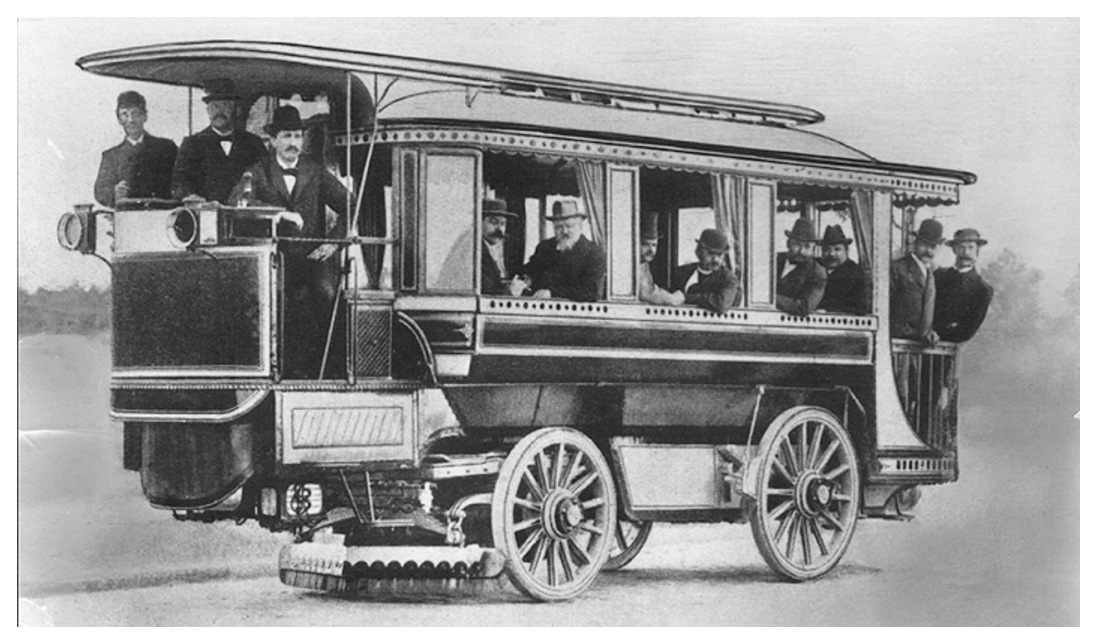
\includegraphics[width=\myFigureStandardWidth]{ersterEbus}
	\caption[Der Berliner Elektrobus 1898]{Der Berliner Elektrobus 1898. Quelle: \texttt{omnibusarchiv.de}}
	\label{abb_ersterEbus}
\end{figure}

\begin{quote}
	"`Das Urteil über die im Berliner Verkehrsleben bisher erschienenen elektrischen Omnibusse muß also dahin zusammengefaßt werden, daß dieselben zwar schon recht anerkennenswerte Leistungen auf dem Gebiete der elektrischen Fahrzeuge darstellen, jedoch von dem wünschenswerten Grade von Vollkommenheit noch ziemlich weit entfernt und bei dem jetzigen Stande der Technik zur Durchführung eines fahrplanmäßigen Omnibusbetriebes noch nicht geeignet sind."'~\cite{ersterEbus}
\end{quote}

Mit der Entwicklung zuverlässiger Verbrennungsmotoren rückte der batteriebetriebene Elektrobus für die nächsten Jahrzehnte in den Hintergrund. Der Einsatz von Bussen mit Schwungradspeichern in der Schweiz~\cite{tub_aleph001746639}[S. 216] und ein Testbetrieb mit Bleiakkus in einem Anhänger hinter dem Bus in Mönchengladbach~\cite{tub_aleph001746639}[S. 170] zeigten, dass die Speichertechnologie noch nicht ausgereift war. In den USA wurden in den neunziger Jahren Elektrobusse in Chattanooga eingesetzt, aber auch hier war der Einsatz auf kleine Busse und kurze Linien begrenzt~\cite{chattanoogaDOE}.

Mit der Entwicklung von preiswerten Lithium-Ionen-Akkus und Superkondensatoren nach der Jahrtausendwende können inzwischen auch große Busse und lange Buslinien elektrisch befahren werden. Parallel wurden leistungsfähige Ladetechnologien entwickelt, mit denen Busse nicht nur im Depot, sondern auch an End- oder Unterwegshaltestellen aufgeladen werden können.

\section{Der Berliner Elektrobus}
Im Jahr 2015 kehrt der Elektrobus nun nach 116 Jahren in den Berliner Linienverkehr zurück. Statt umgerüsteten Pferdekutschen und Bleibatterien werden nun Stadtbusse von Solaris und schnellladefähige Lithium-Titanat-Batterien verwendet. Der Bus ist in Abbildung \ref{abb_ebus2015} zu sehen. Die Berliner Verkehrsbetriebe (BVG) haben sich für ein induktives Schnellladesystem entschieden, mit dem die Busse an den Endhaltestellen in vier bis sieben Minuten aufgeladen werden können~\cite{ebus2015}. Die Technische Universität Berlin ist für die wissenschaftliche Begleitung dieses Projektes verantwortlich.

Die vorliegende Bachelorarbeit entstand im Rahmen dieser Begleitforschung des E-Bus-Projektes und im Zusammenhang mit dem Promotionsvorhaben von Tu-Anh Ly, dessen Ziel die Entwicklung einer methodischen und gesamtheitlichen Bewertung von Systemkonzepten für die Elektrifizierung von Stadtbussen ist.   

\begin{figure}\centering
	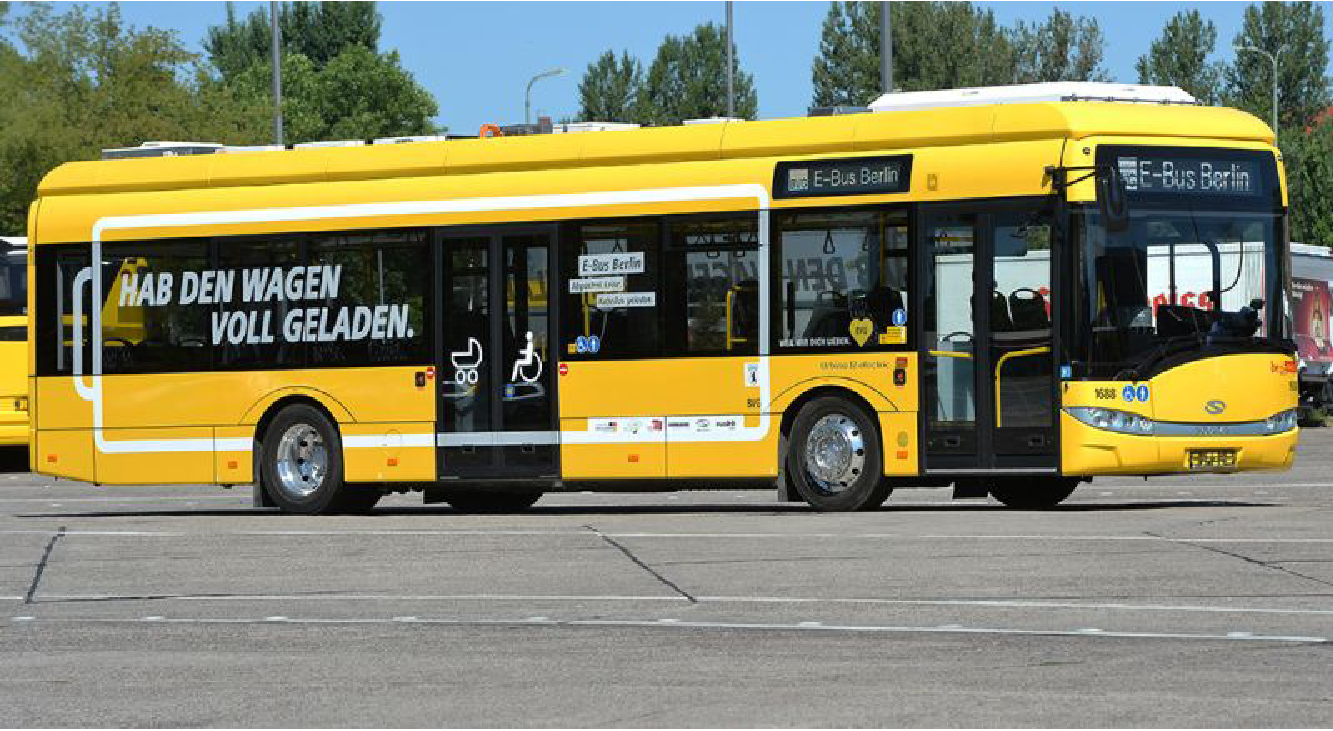
\includegraphics[width=\myFigureStandardWidth]{ebus2015}
	\caption[Der Berliner Elektrobus 2015]{Der Berliner Elektrobus 2015. Quelle: Oliver Lang / BVG}
	\label{abb_ebus2015}
\end{figure}

\section{Problemstellung der vorliegenden Arbeit}
\label{abs_problem}
Es existiert eine Vielzahl von Ladesystemen, Speichertechnologien und Ladestrategien. Der Bus kann konduktiv oder induktiv, manuell oder automatisch sowie bei Stillstand oder während der Fahrt aufgeladen werden. Es gibt viele verschiedene Batterietypen, die verschiedene chemische Reaktionen verwenden. Der Aufladevorgang kann über Nacht im Depot oder an den Endhaltestellen erfolgen. Die Vor- und Nachteile von verschiedenen Technologiekombinationen wirken sich bei unterschiedlichen Streckenführungen unterschiedlich aus. Von daher soll in dieser Arbeit die folgende Frage beantwortet werden:
\begin{quote}
	Welche Kombination von Ladesystem, Speichertechnologie und Ladestrategie ist für welche Buslinie am besten geeignet?
\end{quote}

\section{Methodik}
Um die in Abschnitt \ref{abs_problem} gestellte Frage beantworten zu können, werden zunächst detaillierte Daten zu den existierenden Ladesystemen und Speichertechnologien zusammengestellt. Es wird untersucht, welches Ladesystem für welche Ladestrategie geeignet ist und es werden Buslinien identifiziert, die als geeignete Beispiele für Modellrechnungen dienen können.

Um die Stärken und Schwächen einer Kombination von Ladesystem und Speichertechnologie auf einer bestimmten Buslinie beschreiben zu können, werden relevante Parameter wie Energieverbrauch, Masse, Ladezeit usw. mit einem Simulationsmodell berechnet.

Mit dieser Methode entsteht eine große Menge an Ergebnisdaten. Um diese Menge in aussagekräftige Ergebnisse umzuwandeln, werden die Ergebnisdaten nach systematischen Kriterien zusammengefasst und bewertet.